% Created by tikzDevice version 0.12.3.1 on 2022-03-28 16:56:46
% !TEX encoding = UTF-8 Unicode
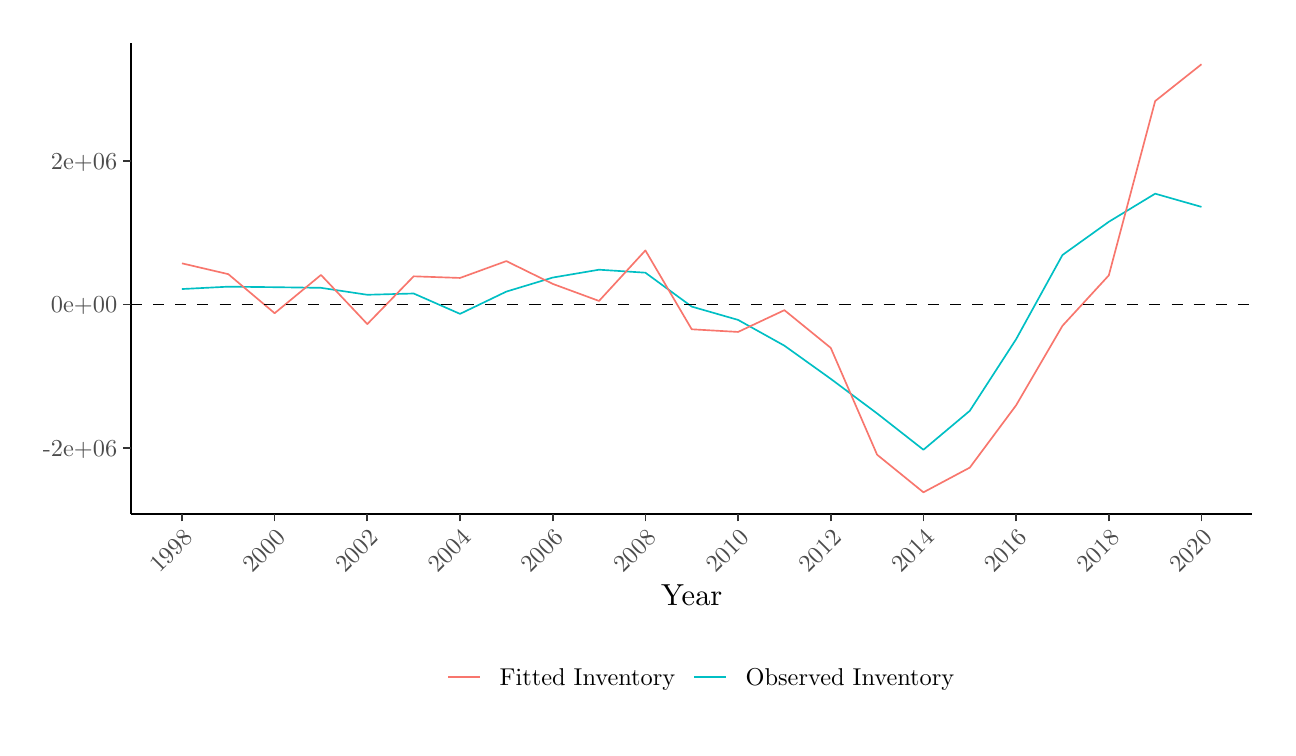
\begin{tikzpicture}[x=1pt,y=1pt]
\definecolor{fillColor}{RGB}{255,255,255}
\path[use as bounding box,fill=fillColor,fill opacity=0.00] (0,0) rectangle (448.07,252.94);
\begin{scope}
\path[clip] (  0.00,  0.00) rectangle (448.07,252.94);
\definecolor{drawColor}{RGB}{255,255,255}
\definecolor{fillColor}{RGB}{255,255,255}

\path[draw=drawColor,line width= 0.6pt,line join=round,line cap=round,fill=fillColor] (  0.00,  0.00) rectangle (448.07,252.94);
\end{scope}
\begin{scope}
\path[clip] ( 37.33, 77.31) rectangle (442.57,247.44);
\definecolor{fillColor}{RGB}{255,255,255}

\path[fill=fillColor] ( 37.33, 77.31) rectangle (442.57,247.44);
\definecolor{drawColor}{RGB}{0,191,196}

\path[draw=drawColor,line width= 0.6pt,line join=round] ( 55.75,158.49) --
	( 72.50,159.35) --
	( 89.24,159.16) --
	(105.99,158.93) --
	(122.73,156.42) --
	(139.48,156.88) --
	(156.23,149.52) --
	(172.97,157.57) --
	(189.72,162.64) --
	(206.46,165.48) --
	(223.21,164.40) --
	(239.95,152.15) --
	(256.70,147.34) --
	(273.44,138.03) --
	(290.19,126.04) --
	(306.94,113.54) --
	(323.68,100.42) --
	(340.43,114.49) --
	(357.17,140.37) --
	(373.92,170.79) --
	(390.66,182.79) --
	(407.41,192.95) --
	(424.15,188.18);
\definecolor{drawColor}{RGB}{248,118,109}

\path[draw=drawColor,line width= 0.6pt,line join=round] ( 55.75,167.78) --
	( 72.50,163.87) --
	( 89.24,149.76) --
	(105.99,163.59) --
	(122.73,145.83) --
	(139.48,163.09) --
	(156.23,162.50) --
	(172.97,168.59) --
	(189.72,160.36) --
	(206.46,154.19) --
	(223.21,172.45) --
	(239.95,143.95) --
	(256.70,142.99) --
	(273.44,150.86) --
	(290.19,137.23) --
	(306.94, 98.63) --
	(323.68, 85.04) --
	(340.43, 93.97) --
	(357.17,116.49) --
	(373.92,145.21) --
	(390.66,163.43) --
	(407.41,226.41) --
	(424.15,239.71);
\definecolor{drawColor}{RGB}{0,0,0}

\path[draw=drawColor,line width= 0.6pt,dash pattern=on 4pt off 4pt ,line join=round] ( 37.33,152.87) -- (442.57,152.87);
\end{scope}
\begin{scope}
\path[clip] (  0.00,  0.00) rectangle (448.07,252.94);
\definecolor{drawColor}{RGB}{0,0,0}

\path[draw=drawColor,line width= 0.6pt,line join=round] ( 37.33, 77.31) --
	( 37.33,247.44);
\end{scope}
\begin{scope}
\path[clip] (  0.00,  0.00) rectangle (448.07,252.94);
\definecolor{drawColor}{gray}{0.30}

\node[text=drawColor,anchor=base east,inner sep=0pt, outer sep=0pt, scale=  0.88] at ( 32.38, 98.05) {-2e+06};

\node[text=drawColor,anchor=base east,inner sep=0pt, outer sep=0pt, scale=  0.88] at ( 32.38,149.84) {0e+00};

\node[text=drawColor,anchor=base east,inner sep=0pt, outer sep=0pt, scale=  0.88] at ( 32.38,201.62) {2e+06};
\end{scope}
\begin{scope}
\path[clip] (  0.00,  0.00) rectangle (448.07,252.94);
\definecolor{drawColor}{gray}{0.20}

\path[draw=drawColor,line width= 0.6pt,line join=round] ( 34.58,101.08) --
	( 37.33,101.08);

\path[draw=drawColor,line width= 0.6pt,line join=round] ( 34.58,152.87) --
	( 37.33,152.87);

\path[draw=drawColor,line width= 0.6pt,line join=round] ( 34.58,204.65) --
	( 37.33,204.65);
\end{scope}
\begin{scope}
\path[clip] (  0.00,  0.00) rectangle (448.07,252.94);
\definecolor{drawColor}{RGB}{0,0,0}

\path[draw=drawColor,line width= 0.6pt,line join=round] ( 37.33, 77.31) --
	(442.57, 77.31);
\end{scope}
\begin{scope}
\path[clip] (  0.00,  0.00) rectangle (448.07,252.94);
\definecolor{drawColor}{gray}{0.20}

\path[draw=drawColor,line width= 0.6pt,line join=round] ( 55.75, 74.56) --
	( 55.75, 77.31);

\path[draw=drawColor,line width= 0.6pt,line join=round] ( 89.24, 74.56) --
	( 89.24, 77.31);

\path[draw=drawColor,line width= 0.6pt,line join=round] (122.73, 74.56) --
	(122.73, 77.31);

\path[draw=drawColor,line width= 0.6pt,line join=round] (156.23, 74.56) --
	(156.23, 77.31);

\path[draw=drawColor,line width= 0.6pt,line join=round] (189.72, 74.56) --
	(189.72, 77.31);

\path[draw=drawColor,line width= 0.6pt,line join=round] (223.21, 74.56) --
	(223.21, 77.31);

\path[draw=drawColor,line width= 0.6pt,line join=round] (256.70, 74.56) --
	(256.70, 77.31);

\path[draw=drawColor,line width= 0.6pt,line join=round] (290.19, 74.56) --
	(290.19, 77.31);

\path[draw=drawColor,line width= 0.6pt,line join=round] (323.68, 74.56) --
	(323.68, 77.31);

\path[draw=drawColor,line width= 0.6pt,line join=round] (357.17, 74.56) --
	(357.17, 77.31);

\path[draw=drawColor,line width= 0.6pt,line join=round] (390.66, 74.56) --
	(390.66, 77.31);

\path[draw=drawColor,line width= 0.6pt,line join=round] (424.15, 74.56) --
	(424.15, 77.31);
\end{scope}
\begin{scope}
\path[clip] (  0.00,  0.00) rectangle (448.07,252.94);
\definecolor{drawColor}{gray}{0.30}

\node[text=drawColor,rotate= 45.00,anchor=base east,inner sep=0pt, outer sep=0pt, scale=  0.88] at ( 60.04, 68.07) {1998};

\node[text=drawColor,rotate= 45.00,anchor=base east,inner sep=0pt, outer sep=0pt, scale=  0.88] at ( 93.53, 68.07) {2000};

\node[text=drawColor,rotate= 45.00,anchor=base east,inner sep=0pt, outer sep=0pt, scale=  0.88] at (127.02, 68.07) {2002};

\node[text=drawColor,rotate= 45.00,anchor=base east,inner sep=0pt, outer sep=0pt, scale=  0.88] at (160.51, 68.07) {2004};

\node[text=drawColor,rotate= 45.00,anchor=base east,inner sep=0pt, outer sep=0pt, scale=  0.88] at (194.00, 68.07) {2006};

\node[text=drawColor,rotate= 45.00,anchor=base east,inner sep=0pt, outer sep=0pt, scale=  0.88] at (227.49, 68.07) {2008};

\node[text=drawColor,rotate= 45.00,anchor=base east,inner sep=0pt, outer sep=0pt, scale=  0.88] at (260.98, 68.07) {2010};

\node[text=drawColor,rotate= 45.00,anchor=base east,inner sep=0pt, outer sep=0pt, scale=  0.88] at (294.48, 68.07) {2012};

\node[text=drawColor,rotate= 45.00,anchor=base east,inner sep=0pt, outer sep=0pt, scale=  0.88] at (327.97, 68.07) {2014};

\node[text=drawColor,rotate= 45.00,anchor=base east,inner sep=0pt, outer sep=0pt, scale=  0.88] at (361.46, 68.07) {2016};

\node[text=drawColor,rotate= 45.00,anchor=base east,inner sep=0pt, outer sep=0pt, scale=  0.88] at (394.95, 68.07) {2018};

\node[text=drawColor,rotate= 45.00,anchor=base east,inner sep=0pt, outer sep=0pt, scale=  0.88] at (428.44, 68.07) {2020};
\end{scope}
\begin{scope}
\path[clip] (  0.00,  0.00) rectangle (448.07,252.94);
\definecolor{drawColor}{RGB}{0,0,0}

\node[text=drawColor,anchor=base,inner sep=0pt, outer sep=0pt, scale=  1.10] at (239.95, 44.09) {Year};
\end{scope}
\begin{scope}
\path[clip] (  0.00,  0.00) rectangle (448.07,252.94);
\definecolor{fillColor}{RGB}{255,255,255}

\path[fill=fillColor] (139.59,  5.50) rectangle (340.31, 30.95);
\end{scope}
\begin{scope}
\path[clip] (  0.00,  0.00) rectangle (448.07,252.94);
\definecolor{drawColor}{RGB}{248,118,109}

\path[draw=drawColor,line width= 0.6pt,line join=round] (152.04, 18.23) -- (163.60, 18.23);
\end{scope}
\begin{scope}
\path[clip] (  0.00,  0.00) rectangle (448.07,252.94);
\definecolor{drawColor}{RGB}{248,118,109}

\path[draw=drawColor,line width= 0.6pt,line join=round] (152.04, 18.23) -- (163.60, 18.23);
\end{scope}
\begin{scope}
\path[clip] (  0.00,  0.00) rectangle (448.07,252.94);
\definecolor{drawColor}{RGB}{0,191,196}

\path[draw=drawColor,line width= 0.6pt,line join=round] (240.94, 18.23) -- (252.50, 18.23);
\end{scope}
\begin{scope}
\path[clip] (  0.00,  0.00) rectangle (448.07,252.94);
\definecolor{drawColor}{RGB}{0,191,196}

\path[draw=drawColor,line width= 0.6pt,line join=round] (240.94, 18.23) -- (252.50, 18.23);
\end{scope}
\begin{scope}
\path[clip] (  0.00,  0.00) rectangle (448.07,252.94);
\definecolor{drawColor}{RGB}{0,0,0}

\node[text=drawColor,anchor=base west,inner sep=0pt, outer sep=0pt, scale=  0.88] at (170.55, 15.20) {Fitted Inventory};
\end{scope}
\begin{scope}
\path[clip] (  0.00,  0.00) rectangle (448.07,252.94);
\definecolor{drawColor}{RGB}{0,0,0}

\node[text=drawColor,anchor=base west,inner sep=0pt, outer sep=0pt, scale=  0.88] at (259.44, 15.20) {Observed Inventory};
\end{scope}
\end{tikzpicture}
